%  Avance final en formato MDPI (Sensors) -- version en espanol para presentacion y revision.
%  Reune las tres etapas de entrenamiento (v1, v4, v5) y la integracion movil (Fase 4 del PPI).
%  Corrige los errores del avance v1 (GPU T4, tiempos en segundos, curva F1, tabla por clase).
%  Compilar: latexmk -pdf main.tex
%=================================================================
\documentclass[sensors,article,submit,pdftex,moreauthors]{Definitions/mdpi}

\firstpage{1}
\makeatletter
\setcounter{page}{\@firstpage}
\makeatother
\pubvolume{1}
\issuenum{1}
\articlenumber{0}
\pubyear{2026}
\copyrightyear{2026}
\datereceived{ }
\daterevised{ }
\dateaccepted{ }
\datepublished{ }

%=================================================================
\usetikzlibrary{positioning,arrows.meta}

%=================================================================
\Title{Detección de Plagas y Enfermedades del Tomate bajo Alta Radiación Solar en el Valle de Majes: Curación del Dataset, Comparación de YOLOv8n, YOLO11n y YOLOv10n, y Despliegue \emph{Offline} en Smartphone}

\Author{Fray Benjamin Kana Chullo $^{1,}$*, Hiram Jeremy Ccoto Cruz $^{1}$ y Angel Rosendo Condori Coaquira $^{1}$}

\AuthorNames{Fray Benjamin Kana Chullo, Hiram Jeremy Ccoto Cruz y Angel Rosendo Condori Coaquira}

\address{%
$^{1}$ \quad Escuela Profesional de Ingeniería de Sistemas, Facultad de Ingeniería y Arquitectura, Universidad Peruana Unión, Juliaca, Perú}

\corres{Correspondencia: fray.kana@upeu.edu.pe}

\abstract{El diagnóstico fitosanitario del tomate en zonas áridas del sur del Perú se ve dificultado por la alta radiación solar, que produce sobreexposición, reflejos y sombras duras en las imágenes RGB. Este trabajo presenta un sistema de visión artificial que detecta cinco clases (mildiu, oídio, mosca blanca, polilla del tomate y hoja sana) en el Valle de Majes, Arequipa, y su integración en una aplicación móvil que funciona sin conexión. El \emph{dataset} se construyó en tres etapas. La primera (v1, 1028 imágenes) alcanzó un mAP@0.5 de 30.6\% en validación, pero una revisión mostró que la división por imagen dejó fotos de la misma planta en entrenamiento y prueba. En la segunda (v4) se revisaron las etiquetas, se dividió por planta y se compararon YOLOv8n, YOLO11n y YOLOv10n con tres semillas: el mAP@0.5 en prueba sin fuga fue de 21.5--24.2\%. En la tercera (v5) se completó el etiquetado de 1966 imágenes de tres sesiones de campo. En las mismas 97 imágenes de prueba, el mAP@0.5:0.95 subió de 9.1--10.4\% a 12.3--13.3\%, mientras que el mAP@0.5 solo mejoró con claridad en YOLOv10n (21.5\% a 28.3\%). Las clases que recibieron más datos mejoraron (hoja sana, mildiu, polilla); oídio y mosca blanca, cuyas cajas miden unos 35 y 10 píxeles a 640~px, no mejoraron. Los tres modelos quedaron empatados dentro de la variación entre semillas. El modelo convertido a TensorFlow Lite (float16, 5.3~MB) procesó una foto en $501 \pm 120$~ms en un Samsung Galaxy A56 sin internet y coincidió con el servidor en la clase principal en el 83.9\% de 192 imágenes. El \emph{dataset}, los \emph{scripts} y los modelos son públicos para que el trabajo pueda reproducirse.}

\keyword{tomate; detección de plagas; YOLOv8; YOLO11; YOLOv10; fuga de datos; TensorFlow Lite; aplicación móvil; radiación solar; Majes}

\begin{document}

%=================================================================
\section{Introducción}

Tradicionalmente, el diagnóstico fitosanitario del tomate se ha basado en inspecciones visuales realizadas por especialistas, un método que depende de personal capacitado y que no siempre está disponible a tiempo en pequeñas y medianas parcelas~\cite{SENASA2020}. En la última década, el aprendizaje profundo ha transformado este diagnóstico: las redes neuronales convolucionales superan el 99\% de precisión en la clasificación de enfermedades foliares con el conjunto PlantVillage~\cite{Mohanty2016}. Sin embargo, esas imágenes tienen fondo uniforme e iluminación controlada, y una revisión de los estudios con \emph{datasets} de campo real advierte que los resultados de laboratorio son sobreoptimistas~\cite{Jelali2024}.

En campo, la detección de objetos permite localizar varias lesiones en una misma imagen. \citet{Fuentes2017} mostraron que detectores como Faster R-CNN y SSD superan a la clasificación simple en tomate, y trabajos recientes optimizan la familia YOLO para esta tarea~\cite{Zhong2024,Wang2025}. El aprendizaje por transferencia es la estrategia habitual cuando los datos propios son escasos~\cite{Mengesha2025,Yadav2025}.

En regiones áridas como el Valle de Majes, la alta irradiancia solar produce píxeles saturados y reflejos especulares en la hoja, que pueden enmascarar el micelio blanco del oídio o el cuerpo de la mosca blanca (\emph{Bemisia tabaci}). Las plagas pequeñas son además un desafío conocido para los detectores de una etapa~\cite{Zhang2024Jute}. Por último, el agricultor no siempre cuenta con señal móvil, por lo que el modelo debe poder ejecutarse en el propio teléfono~\cite{Shafi2023,Ksibi2022,Das2025}.

Un riesgo menos visible es la evaluación. Cuando se fotografía cada planta varias veces y las fotos se reparten al azar, imágenes casi idénticas terminan en entrenamiento y en prueba, y las métricas se inflan~\cite{Kapoor2023}.

\textbf{Contribuciones:}
\begin{enumerate}[leftmargin=*,labelsep=4.9mm]
\item Un \emph{dataset} de campo de 1966 imágenes y 7766 anotaciones de cinco clases, de tres sesiones y tres franjas horarias, dividido por planta y con la fuga de datos medida y corregida, publicado con licencia abierta.
\item Una comparación de YOLOv8n, YOLO11n y YOLOv10n con tres semillas, evaluada en un conjunto de prueba fijo para medir el efecto de ampliar el \emph{dataset}.
\item Un análisis de por qué el modelo no mejora más, basado en el crecimiento de cada clase y en el tamaño de los objetos.
\item La integración del modelo en una aplicación móvil \emph{offline-first}, medida en un teléfono real.
\end{enumerate}

%=================================================================
\section{Materiales y Métodos}

\subsection{Fases de la Investigación}

La propuesta se organiza en cinco fases (Figura~\ref{fig:fases}). Este documento reporta las Fases 1 a 4 completas y la Fase 5 en curso.

\begin{figure}[H]
\centering
\resizebox{\linewidth}{!}{%
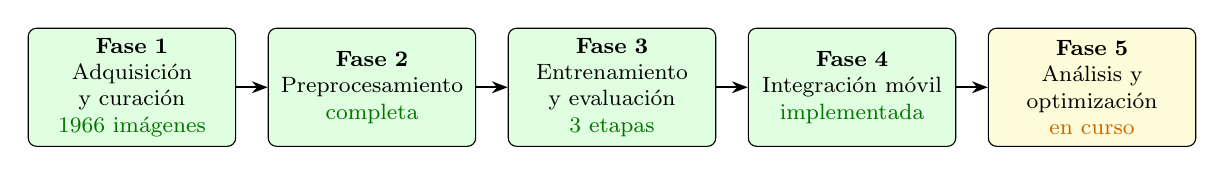
\begin{tikzpicture}[
  font=\footnotesize,
  f/.style={draw, rounded corners=3pt, align=center, text width=24mm, minimum height=15mm},
  arr/.style={-{Stealth[length=2mm]}, thick}
]
\node[f, fill=green!12] (f1) {\textbf{Fase 1}\\Adquisición y curación\\\textcolor{green!45!black}{1966 imágenes}};
\node[f, fill=green!12, right=4mm of f1] (f2) {\textbf{Fase 2}\\Preprocesamiento\\\textcolor{green!45!black}{completa}};
\node[f, fill=green!12, right=4mm of f2] (f3) {\textbf{Fase 3}\\Entrenamiento y evaluación\\\textcolor{green!45!black}{3 etapas}};
\node[f, fill=green!12, right=4mm of f3] (f4) {\textbf{Fase 4}\\Integración móvil\\\textcolor{green!45!black}{implementada}};
\node[f, fill=yellow!15, right=4mm of f4] (f5) {\textbf{Fase 5}\\Análisis y optimización\\\textcolor{orange!80!black}{en curso}};
\draw[arr] (f1) -- (f2); \draw[arr] (f2) -- (f3); \draw[arr] (f3) -- (f4); \draw[arr] (f4) -- (f5);
\end{tikzpicture}}
\caption{Fases metodológicas y estado de avance.\label{fig:fases}}
\end{figure}

\subsection{Fase 1: Adquisición y Curación del Dataset}

Las imágenes se capturaron en el Fundo El Pedregal, Majes, Arequipa, en tres sesiones (3 de mayo, 12 de julio y 29 de julio de 2026), con un Samsung Galaxy A56 5G (cámara de 50~MP), sin flash ni modificación de las plantas. También se extrajeron cuadros de videos cortos. El \emph{dataset} pasó por tres etapas (Tabla~\ref{tab:etapas}).

\begin{table}[H]
\caption{Etapas del \emph{dataset} y del entrenamiento. Imágenes por subconjunto: entrenamiento / validación / prueba.\label{tab:etapas}}
\begin{tabularx}{\textwidth}{lXXX}
\toprule
& \textbf{v1} & \textbf{v4} & \textbf{v5}\\
\midrule
Imágenes & 1028 (720/205/103) & 1021 (715/204/102) & 1966 (1405/381/180)\\
Sesiones & 3 de mayo & 3 de mayo & mayo y julio (3)\\
Etiquetas & originales & revisadas con reglas escritas & etiquetado completo\\
División & por imagen (con fuga) & por planta & por planta + video\\
Formato & estirado a $640\times640$ & sin deformar & sin deformar\\
Modelos & YOLOv8n, 3 configuraciones & YOLOv8n, YOLO11n, YOLOv10n & YOLOv8n, YOLO11n, YOLOv10n\\
Semillas & 1 & 3 & 3\\
GPU & Tesla T4 (Colab) & Tesla T4 (Colab) & RTX 5070 Ti\\
\bottomrule
\end{tabularx}
\end{table}

\textbf{Revisión de la v1.} Se encontraron tres problemas. (i) \emph{Fuga de datos}: las fotos se tomaron en ráfagas alrededor de cada planta y la división se hizo por imagen; al agrupar como misma planta las fotos separadas por menos de 30~s, 65 de 189 plantas tenían imágenes en más de un subconjunto y 82 de las 103 imágenes de prueba tenían una foto de la misma planta en entrenamiento o validación. (ii) \emph{Imágenes deformadas}: la exportación estiró las fotos 3:4 a 1:1. (iii) \emph{Etiquetas inconsistentes}: cajas fuera de la lesión o faltantes.

\textbf{Curación para la v4 y la v5.} Cada imagen se asignó a un grupo de planta (ráfagas de menos de 30~s; los cuadros de un video forman un solo grupo) y los 288 grupos se repartieron completos, 70/20/10 por número de imágenes dentro de cada carpeta horaria. Una revisión posterior encontró 18 casos en que un video se grabó a menos de 30~s de una ráfaga de fotos de la misma planta pero había caído en otro subconjunto; esas 66 imágenes (3.4\%) se movieron al subconjunto de su planta. El \emph{script} de entrenamiento verifica ambas reglas y se detiene si encuentra fuga. Las etiquetas se revisaron con reglas escritas: una caja por lesión, insecto o mina; \texttt{sana} solo para hojas; hojas superpuestas con una caja cada una; y todo lo reconocible en primer plano etiquetado. La Tabla~\ref{tab:dataset} muestra la distribución final.

\begin{table}[H]
\caption{Anotaciones del \emph{dataset} v5 (después de mover las 66 imágenes).\label{tab:dataset}}
\begin{tabularx}{\textwidth}{lCCCC}
\toprule
\textbf{Clase} & \textbf{Entren.} & \textbf{Valid.} & \textbf{Prueba} & \textbf{Total}\\
\midrule
\texttt{sana} & 2344 & 746 & 266 & 3356\\
\texttt{mildiu} (\emph{Phytophthora infestans}) & 1882 & 543 & 273 & 2698\\
\texttt{oidio} & 594 & 206 & 89 & 889\\
\texttt{polilla} (\emph{Tuta absoluta}) & 374 & 71 & 29 & 474\\
\texttt{mosca\_blanca} (\emph{Bemisia tabaci}) & 253 & 62 & 34 & 349\\
\midrule
\textbf{Total} & \textbf{5447} & \textbf{1628} & \textbf{691} & \textbf{7766}\\
\bottomrule
\end{tabularx}
\end{table}

\textbf{Hora real de captura.} La carpeta de cada sesión no siempre coincide con la hora real (por ejemplo, la de las 16:00~h llega hasta las 17:44). Por eso cada imagen se clasificó según la hora de su archivo: mañana (antes de las 11:00, 555 imágenes), mediodía (11:00--13:59, 397) y tarde (desde las 14:00, 1014). En prueba hay 49, 35 y 96 imágenes por franja.

\subsection{Fase 2: Preprocesamiento}

Las versiones de Roboflow de la v4 y la v5 se generaron con orientación automática y \emph{Fit within} $1024\times1024$, sin deformar las fotos y sin aumentos. El aumento de datos lo aplica Ultralytics solo al conjunto de entrenamiento (mosaico, volteo horizontal, escala, traslación y variación HSV por defecto). La Figura~\ref{fig:batch} muestra un lote con sus anotaciones.

\begin{figure}[H]
\centering
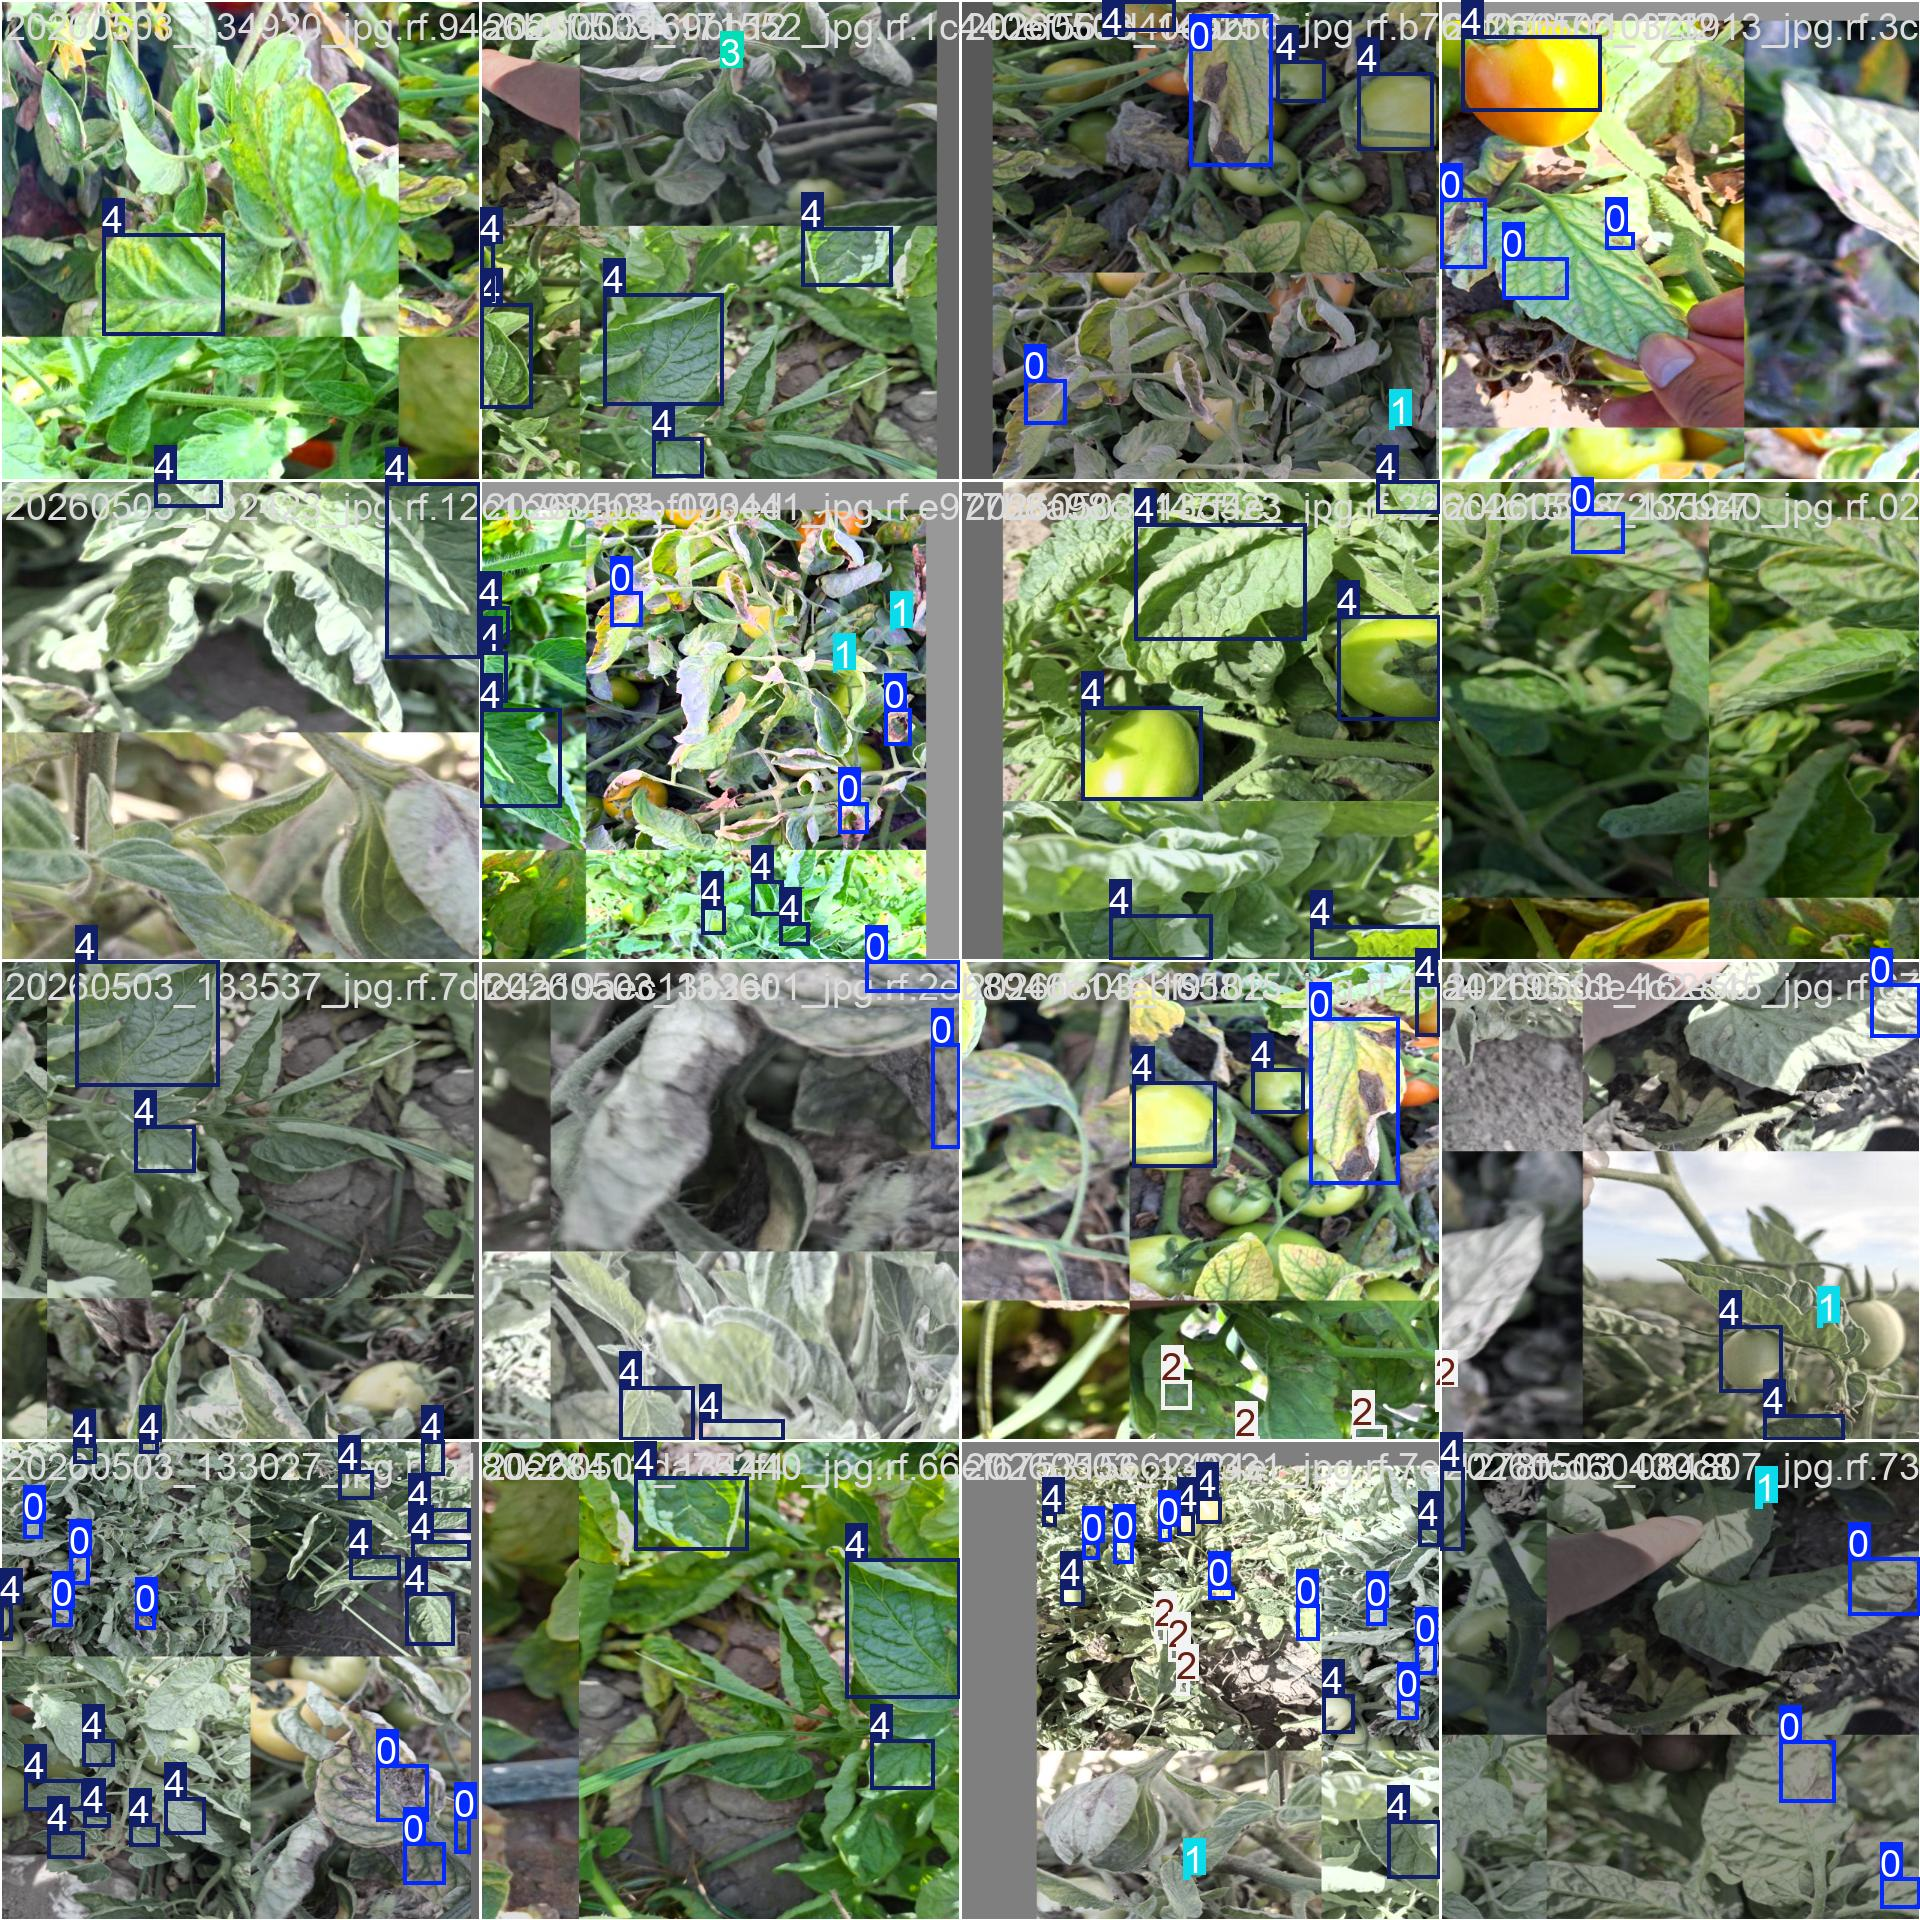
\includegraphics[width=0.72\textwidth]{train_batch2.jpg}
\caption{Lote de entrenamiento con cajas de \texttt{mildiu}, \texttt{oidio}, \texttt{sana} y \texttt{mosca\_blanca}.\label{fig:batch}}
\end{figure}

\subsection{Fase 3: Entrenamiento y Evaluación}

Todos los modelos parten de pesos preentrenados en COCO~\cite{Jocher2023,Jocher2024,Wang2024v10} y se entrenaron a $640\times640$, el tamaño que usa la aplicación.
\begin{itemize}[leftmargin=*,labelsep=4.9mm]
\item \textbf{v1:} YOLOv8n con una semilla en tres configuraciones: 50 épocas (11.8~min), 150 épocas con paciencia 30 (se detuvo en la 139; 33.8~min) y 100 épocas con más variación HSV y rotación de 15° (24.4~min).
\item \textbf{v4:} YOLOv8n, YOLO11n y YOLOv10n con las semillas 0, 1 y 2; hasta 150 épocas con paciencia 30 y \emph{batch} 16.
\item \textbf{v5:} los mismos tres modelos y semillas; hasta 200 épocas con paciencia 50, \emph{batch} 32, tasa de aprendizaje coseno, precisión mixta y cierre del mosaico en las últimas 15 épocas. Cada corrida tardó entre 6 y 12~min.
\end{itemize}

\textbf{Protocolo de evaluación (v4 y v5).} El mejor modelo se elige con el mAP@0.5:0.95 de validación, nunca con prueba. Se reportan mAP@0.5, mAP@0.5:0.95, precisión y \emph{recall} en prueba, total, por clase y por franja horaria, como media $\pm$ desviación estándar de las tres semillas. Para medir el efecto de ampliar el \emph{dataset}, las versiones se comparan en un \textbf{test fijo}: las 102 imágenes de prueba de la v4, de las cuales 97 siguen en prueba en la v5 (las otras 5 salieron por la corrección de video). Además se calcula el \textbf{acierto de la clase principal} con las mismas reglas de la aplicación (detección de mayor confianza con confianza 0.30, IoU 0.45 y NMS agnóstica; sin detecciones cuenta como \texttt{sana}), con intervalo de confianza de Wilson al 95\%.

\subsection{Fase 4: Integración del Modelo en el Móvil}

El sistema sigue la arquitectura híbrida de inferencia dual del PPI (Figura~\ref{fig:arq}).

\begin{figure}[H]
\centering
\resizebox{\linewidth}{!}{%
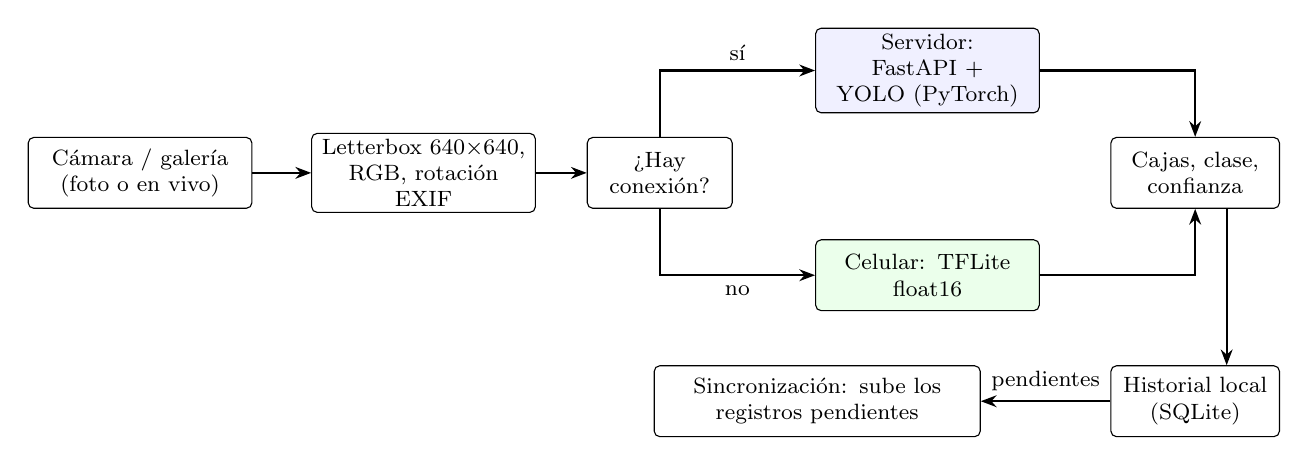
\begin{tikzpicture}[
  font=\footnotesize,
  box/.style={draw, rounded corners=2pt, align=center, minimum height=9mm, text width=27mm, inner sep=2pt, fill=white},
  arr/.style={-{Stealth[length=2mm]}, thick}
]
\node[box] (cam) at (0,0) {Cámara / galería\\(foto o en vivo)};
\node[box] (pre) at (3.6,0) {Letterbox 640$\times$640,\\RGB, rotación EXIF};
\node[box, text width=17mm] (route) at (6.6,0) {¿Hay\\conexión?};
\node[box, fill=blue!6] (srv) at (10,1.3) {Servidor: FastAPI +\\YOLO (PyTorch)};
\node[box, fill=green!8] (tfl) at (10,-1.3) {Celular: TFLite\\float16};
\node[box, text width=20mm] (res) at (13.4,0) {Cajas, clase,\\confianza};
\node[box, text width=20mm] (db) at (13.4,-2.9) {Historial local\\(SQLite)};
\node[box, text width=40mm] (sync) at (8.6,-2.9) {Sincronización: sube los\\registros pendientes};
\draw[arr] (cam) -- (pre);
\draw[arr] (pre) -- (route);
\draw[arr] (route.north) |- node[pos=0.75, above]{sí} (srv.west);
\draw[arr] (route.south) |- node[pos=0.75, below]{no} (tfl.west);
\draw[arr] (srv.east) -| (res.north);
\draw[arr] (tfl.east) -| (res.south);
\draw[arr] (res.south) ++(4mm,0) -- ([xshift=4mm]db.north);
\draw[arr] (db) -- node[above]{pendientes} (sync);
\end{tikzpicture}}
\caption{Arquitectura \emph{offline-first}. Con conexión, la imagen se analiza en el servidor; sin conexión, el modelo TFLite se ejecuta en el teléfono y el registro se sube después.\label{fig:arq}}
\end{figure}

\begin{itemize}[leftmargin=*,labelsep=4.9mm]
\item \textbf{Servidor:} API REST con FastAPI que ejecuta el modelo con Ultralytics. Las imágenes se corrigen según su orientación EXIF y se pasan en RGB, con confianza 0.30, IoU 0.45 y NMS agnóstica. Los usuarios se autentican con JWT.
\item \textbf{Conversión:} el modelo se exporta a ONNX (opset 17) y se convierte a TensorFlow Lite con onnx2tf en float16. La salida es un tensor $1\times9\times8400$ (cuatro coordenadas y cinco clases).
\item \textbf{Aplicación (Flutter):} reproduce el preprocesamiento del servidor (\emph{letterbox} con gris 114, mismos umbrales y NMS) y ejecuta la inferencia en un \emph{isolate}. Tiene modo foto y modo en vivo.
\item \textbf{Persistencia y sincronización:} cada resultado se guarda en SQLite con sus cajas, su origen y la versión del modelo; lo analizado sin conexión se sincroniza al volver la señal.
\end{itemize}

\textbf{Pruebas en el teléfono} (Samsung Galaxy A56 5G, Exynos 1580, 12~GB, Android~16). Una prueba automatizada pasó 192 imágenes de campo por el mismo código de detección de la aplicación y midió el tiempo desde los bytes JPEG hasta las cajas finales (P1). Las mismas imágenes se procesaron con el modelo del servidor para comparar la clase principal y las cajas, con misma clase e IoU $\geq 0.5$ (P2). También se midieron el modo en vivo (P3), el funcionamiento sin conexión con sincronización posterior (P4) y el análisis en el servidor (P5).

\subsection{Disponibilidad de los Datos y Reproducibilidad}\label{sec:repro}

Todo el material necesario para repetir los experimentos es público (Tabla~\ref{tab:repro}). El \emph{dataset} está en Roboflow Universe con licencia CC~BY~4.0~\cite{Dataset2026}; cada etapa corresponde a una versión fija: la versión~1 (1021 imágenes) para la v4 y la versión~2 (1966 imágenes) para la v5. El \emph{script} \texttt{entrenar\_yolo.py} descomprime el \emph{dataset}, comprueba el orden de las clases, los conteos y la ausencia de fuga, aplica los 66 movimientos de la corrección de video (lista en \texttt{movimientos\_split\_v5.csv}), entrena los tres modelos con las semillas 0, 1 y 2 y evalúa en prueba, por franja horaria y en el test fijo (lista en \texttt{test\_fijo\_v4.txt}). Se usaron Ultralytics 8.4.82 y PyTorch 2.12 con CUDA 13.2. Como el entrenamiento de la v5 usó \texttt{deterministic=False} por velocidad, una nueva ejecución puede diferir ligeramente; por eso se reportan tres semillas.

\begin{table}[H]
\caption{Recursos públicos del trabajo.\label{tab:repro}}
\begin{adjustwidth}{-\extralength}{0cm}
\begin{tabularx}{\fulllength}{lX}
\toprule
\textbf{Recurso} & \textbf{Enlace}\\
\midrule
\emph{Dataset} (todas las versiones) & \url{https://universe.roboflow.com/fray-hxtls/plagas-tomate-majes-v2}\\
Versión 2 (v5: 1966 imágenes) & \url{https://universe.roboflow.com/fray-hxtls/plagas-tomate-majes-v2/dataset/2}\\
Versión 1 (v4: 1021 imágenes) & \url{https://universe.roboflow.com/fray-hxtls/plagas-tomate-majes-v2/dataset/1}\\
\emph{Scripts}, resultados y modelos & \url{https://github.com/fraykanachullo/trabajoinvestigacionTomate}\\
Servidor (FastAPI) & \url{https://github.com/fraykanachullo/backentTomate}\\
Aplicación móvil (Flutter) & \url{https://github.com/fraykanachullo/frontendTomate}\\
\bottomrule
\end{tabularx}
\end{adjustwidth}
\end{table}

%=================================================================
\section{Resultados}

\subsection{Etapa v1: Resultados Preliminares}

Los tres experimentos de la v1 empataron: su mejor mAP@0.5 en validación fue 30.2\%, 30.6\% y 30.2\% (Tabla~\ref{tab:v1}). La pérdida de clasificación en validación subió desde la época $\sim$50 mientras la de entrenamiento seguía bajando, una señal de sobreajuste. Estos valores están inflados por la fuga de datos; por ejemplo, \texttt{polilla} obtuvo 63--66\% con solo 25 cajas en validación.

\begin{table}[H]
\caption{YOLOv8n en la v1: mejor época en validación (con fuga de datos).\label{tab:v1}}
\begin{tabularx}{\textwidth}{lCCC}
\toprule
& \textbf{Exp. 1 (50 ép.)} & \textbf{Exp. 2 (139 ép.)} & \textbf{Exp. 3 (HSV + rotación)}\\
\midrule
mAP@0.5 & 30.2\% & 30.6\% & 30.2\%\\
mAP@0.5:0.95 & 13.6\% & 14.0\% & 13.3\%\\
AP@0.5 \texttt{polilla} / \texttt{sana} & 63.5 / 46.4\% & 66.1 / 46.0\% & 63.4 / 48.5\%\\
AP@0.5 \texttt{mildiu} / \texttt{mosca\_blanca} / \texttt{oidio} & 22.6 / 10.0 / 8.4\% & 16.5 / 13.7 / 6.5\% & 16.5 / 9.4 / 6.8\%\\
Tiempo de entrenamiento (T4) & 11.8 min & 33.8 min & 24.4 min\\
\bottomrule
\end{tabularx}
\end{table}

\subsection{Etapa v4: Prueba sin Fuga de Datos}

Con la división por planta, el mAP@0.5 en prueba bajó a 21.5--24.2\% (Tabla~\ref{tab:v4v5}), lo que confirma que la v1 estaba inflada. El caso más claro es \texttt{polilla}, que cayó de $\sim$65\% a 15--25\%. YOLO11n fue el mejor en validación, y el modelo elegido (YOLO11n, semilla 1) obtuvo 23.9\% de mAP@0.5 en prueba y 67.6\% de acierto de la clase principal (IC95\%: 58--76\%).

\subsection{Etapa v5: Efecto de Completar el Etiquetado}\label{sec:v5}

La Tabla~\ref{tab:v4v5} y la Figura~\ref{fig:modelos} comparan la v4 y la v5. En validación y en la prueba completa la v5 obtiene valores mucho más altos, pero esos conjuntos cambiaron (incluyen las sesiones de julio). En el test fijo, que es la comparación justa, el mAP@0.5:0.95 sube entre 1.9 y 4.2 puntos en los tres modelos; el mAP@0.5 solo mejora con claridad en YOLOv10n (+6.8), y el acierto de la clase principal no cambia de forma significativa.

\begin{table}[H]
\caption{Comparación v4 frente a v5 (media $\pm$ desviación de 3 semillas, en \%). La prueba completa tiene 102 imágenes en la v4 y 180 en la v5; el test fijo tiene las mismas 97 imágenes en ambas.\label{tab:v4v5}}
\begin{adjustwidth}{-\extralength}{0cm}
\begin{tabularx}{\fulllength}{lCCCCCC}
\toprule
& \multicolumn{2}{c}{\textbf{YOLOv8n}} & \multicolumn{2}{c}{\textbf{YOLO11n}} & \multicolumn{2}{c}{\textbf{YOLOv10n}}\\
\textbf{Métrica} & \textbf{v4} & \textbf{v5} & \textbf{v4} & \textbf{v5} & \textbf{v4} & \textbf{v5}\\
\midrule
mAP@0.5 validación & $28.7 \pm 0.9$ & $38.5 \pm 0.4$ & $30.4 \pm 0.7$ & $34.7 \pm 1.9$ & $27.7 \pm 1.5$ & $35.5 \pm 3.0$\\
mAP@0.5:0.95 validación & $12.3 \pm 0.1$ & $19.1 \pm 0.5$ & $12.8 \pm 0.5$ & $17.4 \pm 0.7$ & $11.5 \pm 0.5$ & $17.9 \pm 1.5$\\
mAP@0.5 prueba completa & $23.8 \pm 3.2$ & $33.6 \pm 2.4$ & $24.2 \pm 0.6$ & $32.1 \pm 4.0$ & $21.5 \pm 2.3$ & $36.3 \pm 1.1$\\
\textbf{mAP@0.5 test fijo} & $23.8 \pm 3.2$ & $\mathbf{25.1 \pm 0.6}$ & $24.2 \pm 0.6$ & $\mathbf{24.6 \pm 0.8}$ & $21.5 \pm 2.3$ & $\mathbf{28.3 \pm 0.9}$\\
\textbf{mAP@0.5:0.95 test fijo} & $10.4 \pm 1.9$ & $\mathbf{12.3 \pm 0.3}$ & $10.1 \pm 0.8$ & $\mathbf{12.3 \pm 0.8}$ & $9.1 \pm 1.0$ & $\mathbf{13.3 \pm 1.0}$\\
Acierto clase principal, test fijo & $60.8 \pm 4.3$ & $58.1 \pm 10.1$ & $58.8 \pm 9.4$ & $60.8 \pm 7.4$ & $55.9 \pm 15.2$ & $63.2 \pm 12.1$\\
\bottomrule
\end{tabularx}
\end{adjustwidth}
\end{table}

\begin{figure}[H]
\centering
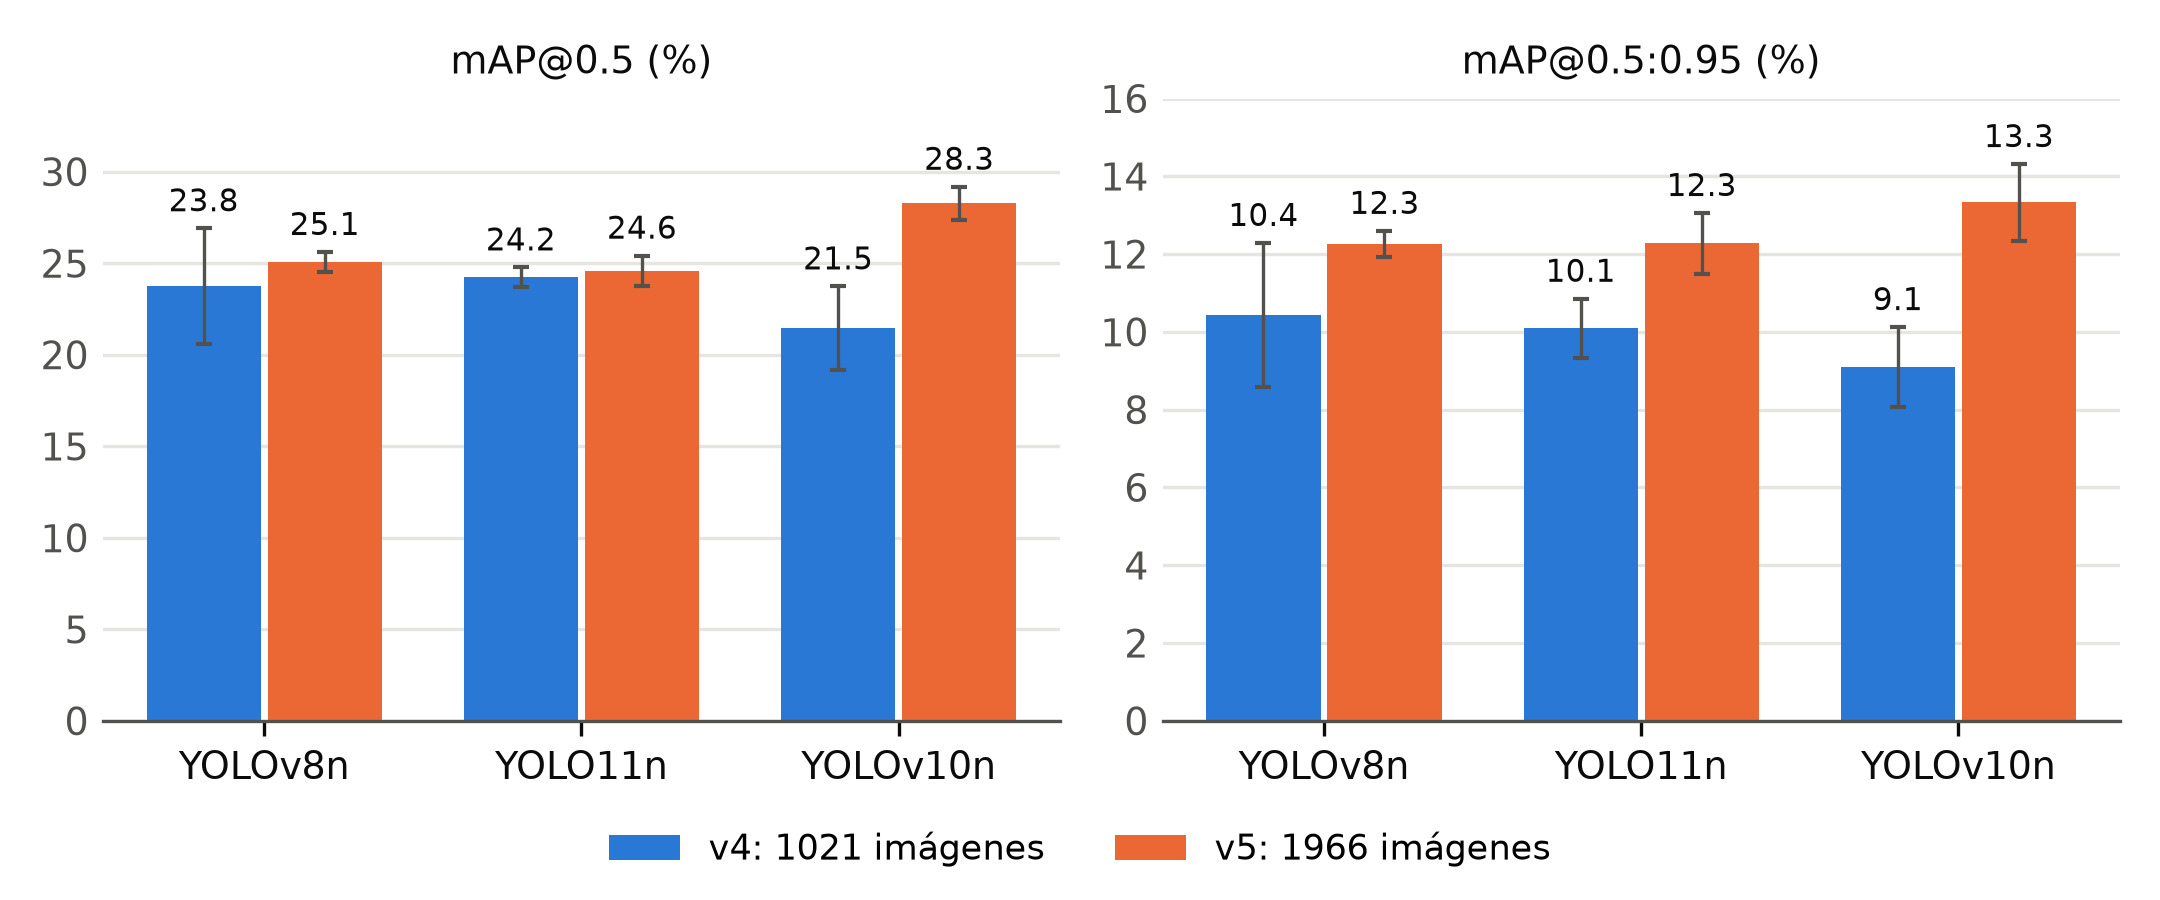
\includegraphics[width=0.92\textwidth]{fig_v4_v5_modelos.png}
\caption{mAP en el test fijo (las mismas 97 imágenes) para la v4 y la v5. Las barras de error son la desviación entre las tres semillas.\label{fig:modelos}}
\end{figure}

\textbf{Por clase} (Figura~\ref{fig:clases}), el resultado sigue al crecimiento de los datos: \texttt{sana} (+167\% de cajas de entrenamiento), \texttt{mildiu} (+93\%) y \texttt{polilla} (+290\%) mejoraron, mientras que \texttt{mosca\_blanca} (+23\%) y \texttt{oidio} (+8\%) empeoraron. En la prueba completa, con 29 cajas de polilla en lugar de 9, esta clase llega a 39--62\% de AP@0.5.

\begin{figure}[H]
\centering
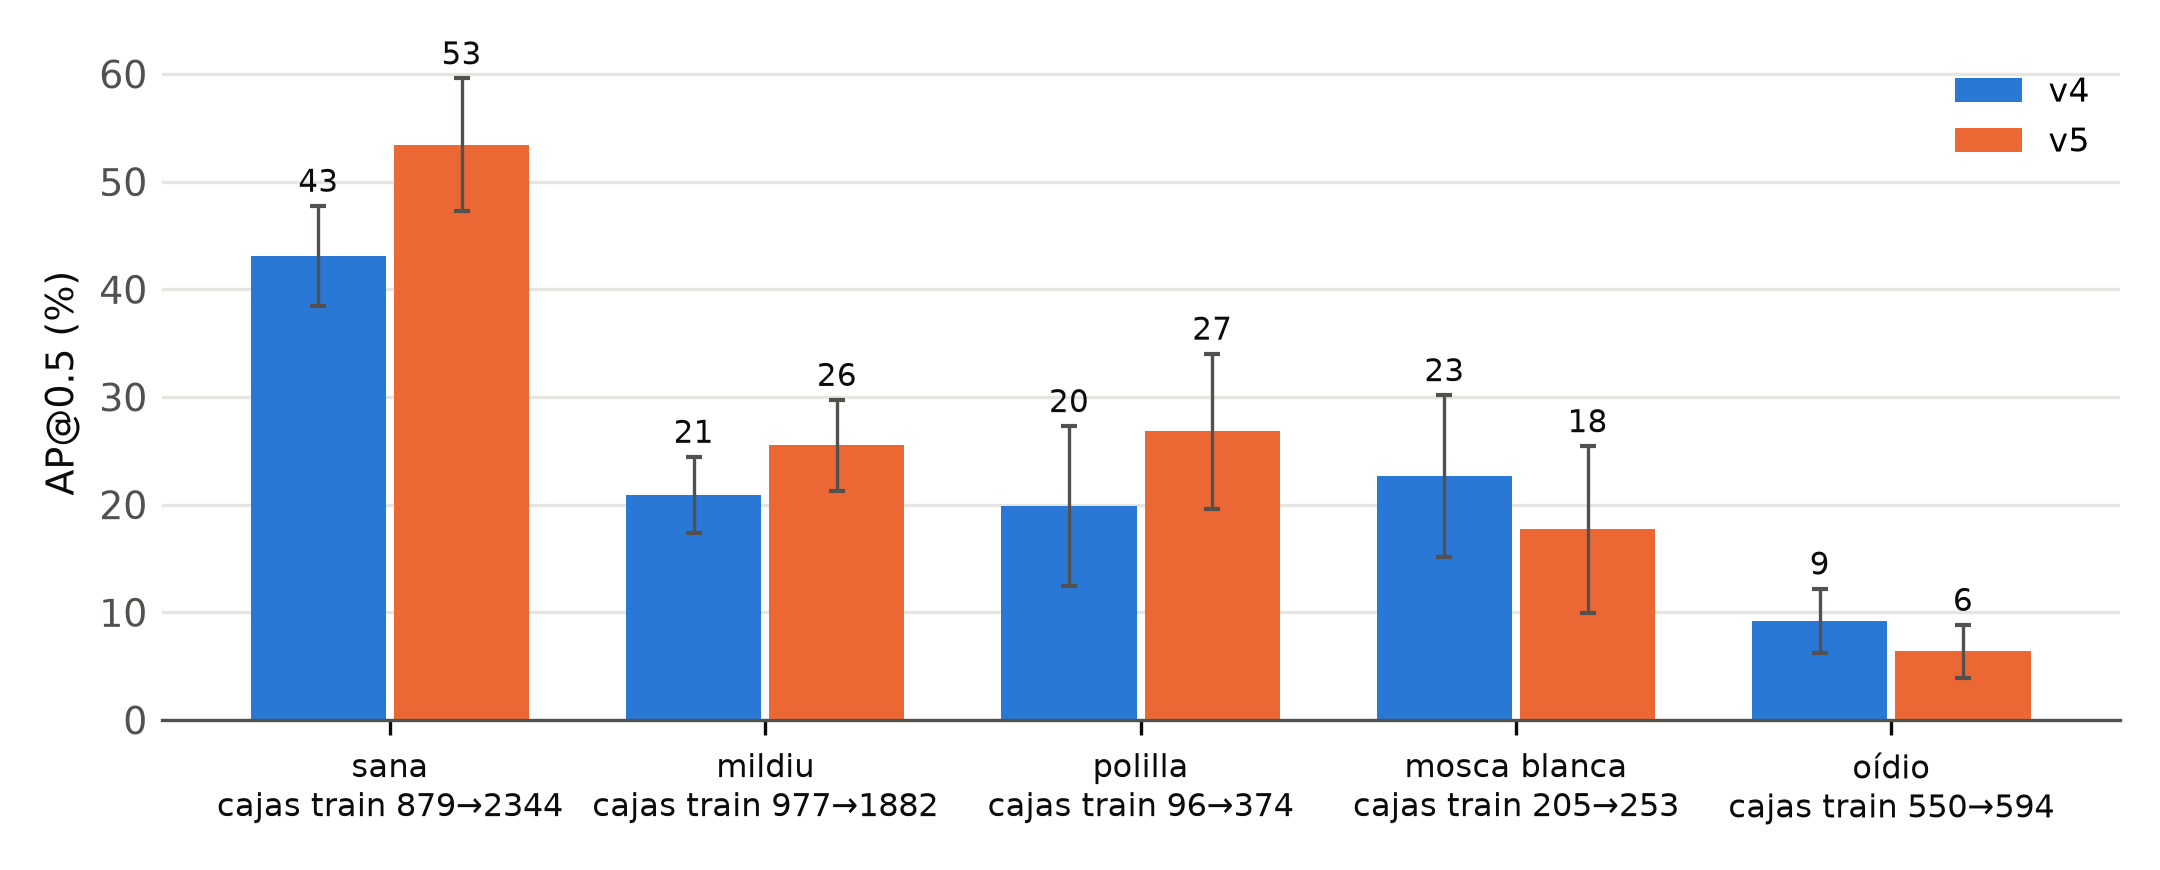
\includegraphics[width=0.92\textwidth]{fig_v4_v5_clases.png}
\caption{AP@0.5 por clase en el test fijo (media de las 9 corridas de cada versión) y crecimiento de las cajas de entrenamiento de cada clase entre la v4 y la v5.\label{fig:clases}}
\end{figure}

\textbf{Tamaño de los objetos.} La Tabla~\ref{tab:tamano} muestra el área de las cajas en la imagen. A 640~px, una mosca blanca típica mide unos 10~píxeles de lado, por debajo de los 16~px que exige la regla de etiquetado, y el 10\% más pequeño de las cajas de oídio mide unos 17~px. Las cajas de mildiu son de lesión, más pequeñas que una hoja sana; solo 8 de 1052 imágenes (1\%) mezclan cajas muy pequeñas y muy grandes, por lo que no hay indicios de que se haya mezclado el criterio de mancha con el de hoja entera.

\begin{table}[H]
\caption{Tamaño de las cajas en el \emph{dataset} v5 (área en \% de la imagen; lado aproximado a 640~px).\label{tab:tamano}}
\begin{tabularx}{\textwidth}{lCCCC}
\toprule
\textbf{Clase} & \textbf{Mediana} & \textbf{Percentil 10} & \textbf{Cajas < 1\% de la imagen} & \textbf{Lado típico}\\
\midrule
\texttt{mosca\_blanca} & 0.03\% & 0.01\% & 99\% & $\sim$10 px\\
\texttt{oidio} & 0.40\% & 0.09\% & 79\% & $\sim$35 px\\
\texttt{polilla} & 0.84\% & 0.20\% & 55\% & $\sim$50 px\\
\texttt{mildiu} & 1.25\% & 0.24\% & 43\% & $\sim$60 px\\
\texttt{sana} & 2.56\% & 0.75\% & 16\% & $\sim$90 px\\
\bottomrule
\end{tabularx}
\end{table}

\textbf{Franjas horarias.} En la prueba de la v5 el mAP@0.5 fue de 20--23\% en la mañana, 23--26\% al mediodía y 37--42\% en la tarde. El acierto de la clase principal muestra el orden contrario: 80\% en la mañana, 53--65\% al mediodía y 47--52\% en la tarde. Las franjas están mezcladas con la sesión y con las clases presentes (la tarde de julio concentra la polilla y la mañana incluye la sesión del 12 de julio), por lo que todavía no permiten aislar el efecto de la radiación solar.

\textbf{Modelo elegido.} Por validación se eligió YOLOv8n, semilla 2 (mAP@0.5:0.95 de 19.6\% en validación). La Tabla~\ref{tab:elegidos} lo compara con el modelo de la v4 en la prueba de 180 imágenes, evaluados con las mismas reglas. La Figura~\ref{fig:v5} muestra sus curvas de entrenamiento y la matriz de confusión.

\begin{table}[H]
\caption{Modelo de la v4 frente al de la v5 en la prueba de 180 imágenes (en \%).\label{tab:elegidos}}
\begin{adjustwidth}{-\extralength}{0cm}
\begin{tabularx}{\fulllength}{lCCCCCC}
\toprule
\textbf{Modelo} & \textbf{mAP@0.5} & \textbf{mAP@0.5:0.95} & \textbf{Acierto} & \textbf{AP sana} & \textbf{AP mosca blanca} & \textbf{AP oídio}\\
\midrule
v4: YOLO11n, semilla 1 & 27.8 & 12.0 & 66.1 (119/180) & 52.1 & 16.9 & 11.4\\
v5: YOLOv8n, semilla 2 & 30.9 & 14.6 & 63.9 (115/180) & 68.6 & 22.0 & 5.0\\
\bottomrule
\end{tabularx}
\end{adjustwidth}
\end{table}

\begin{figure}[H]
\centering
\begin{tabular}{@{}c@{\hspace{3mm}}c@{}}
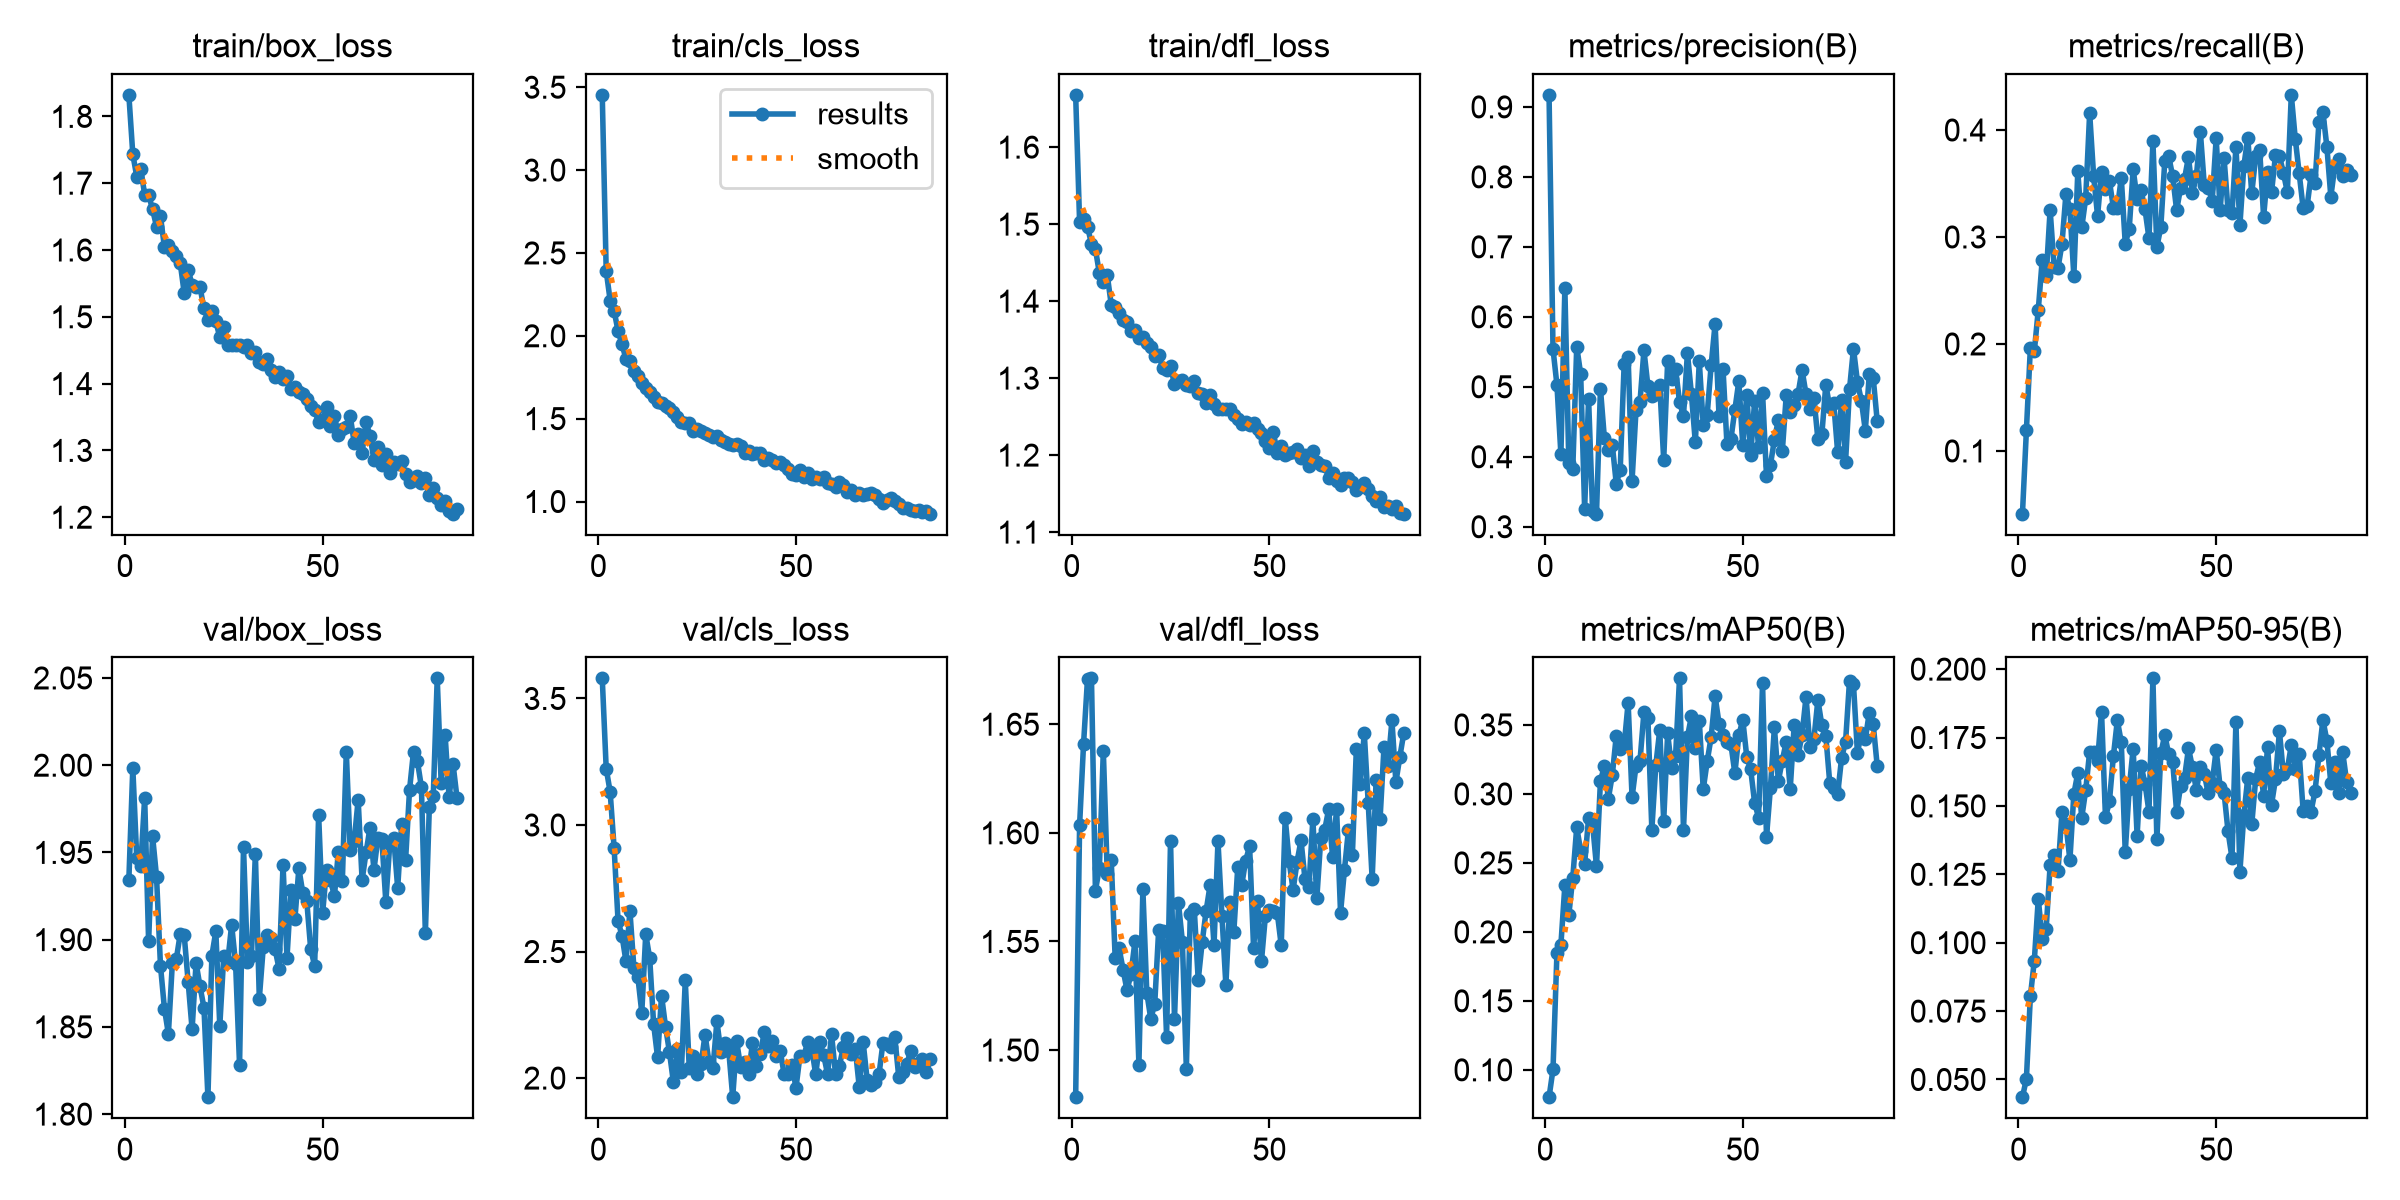
\includegraphics[width=0.56\textwidth]{results_v5.png} &
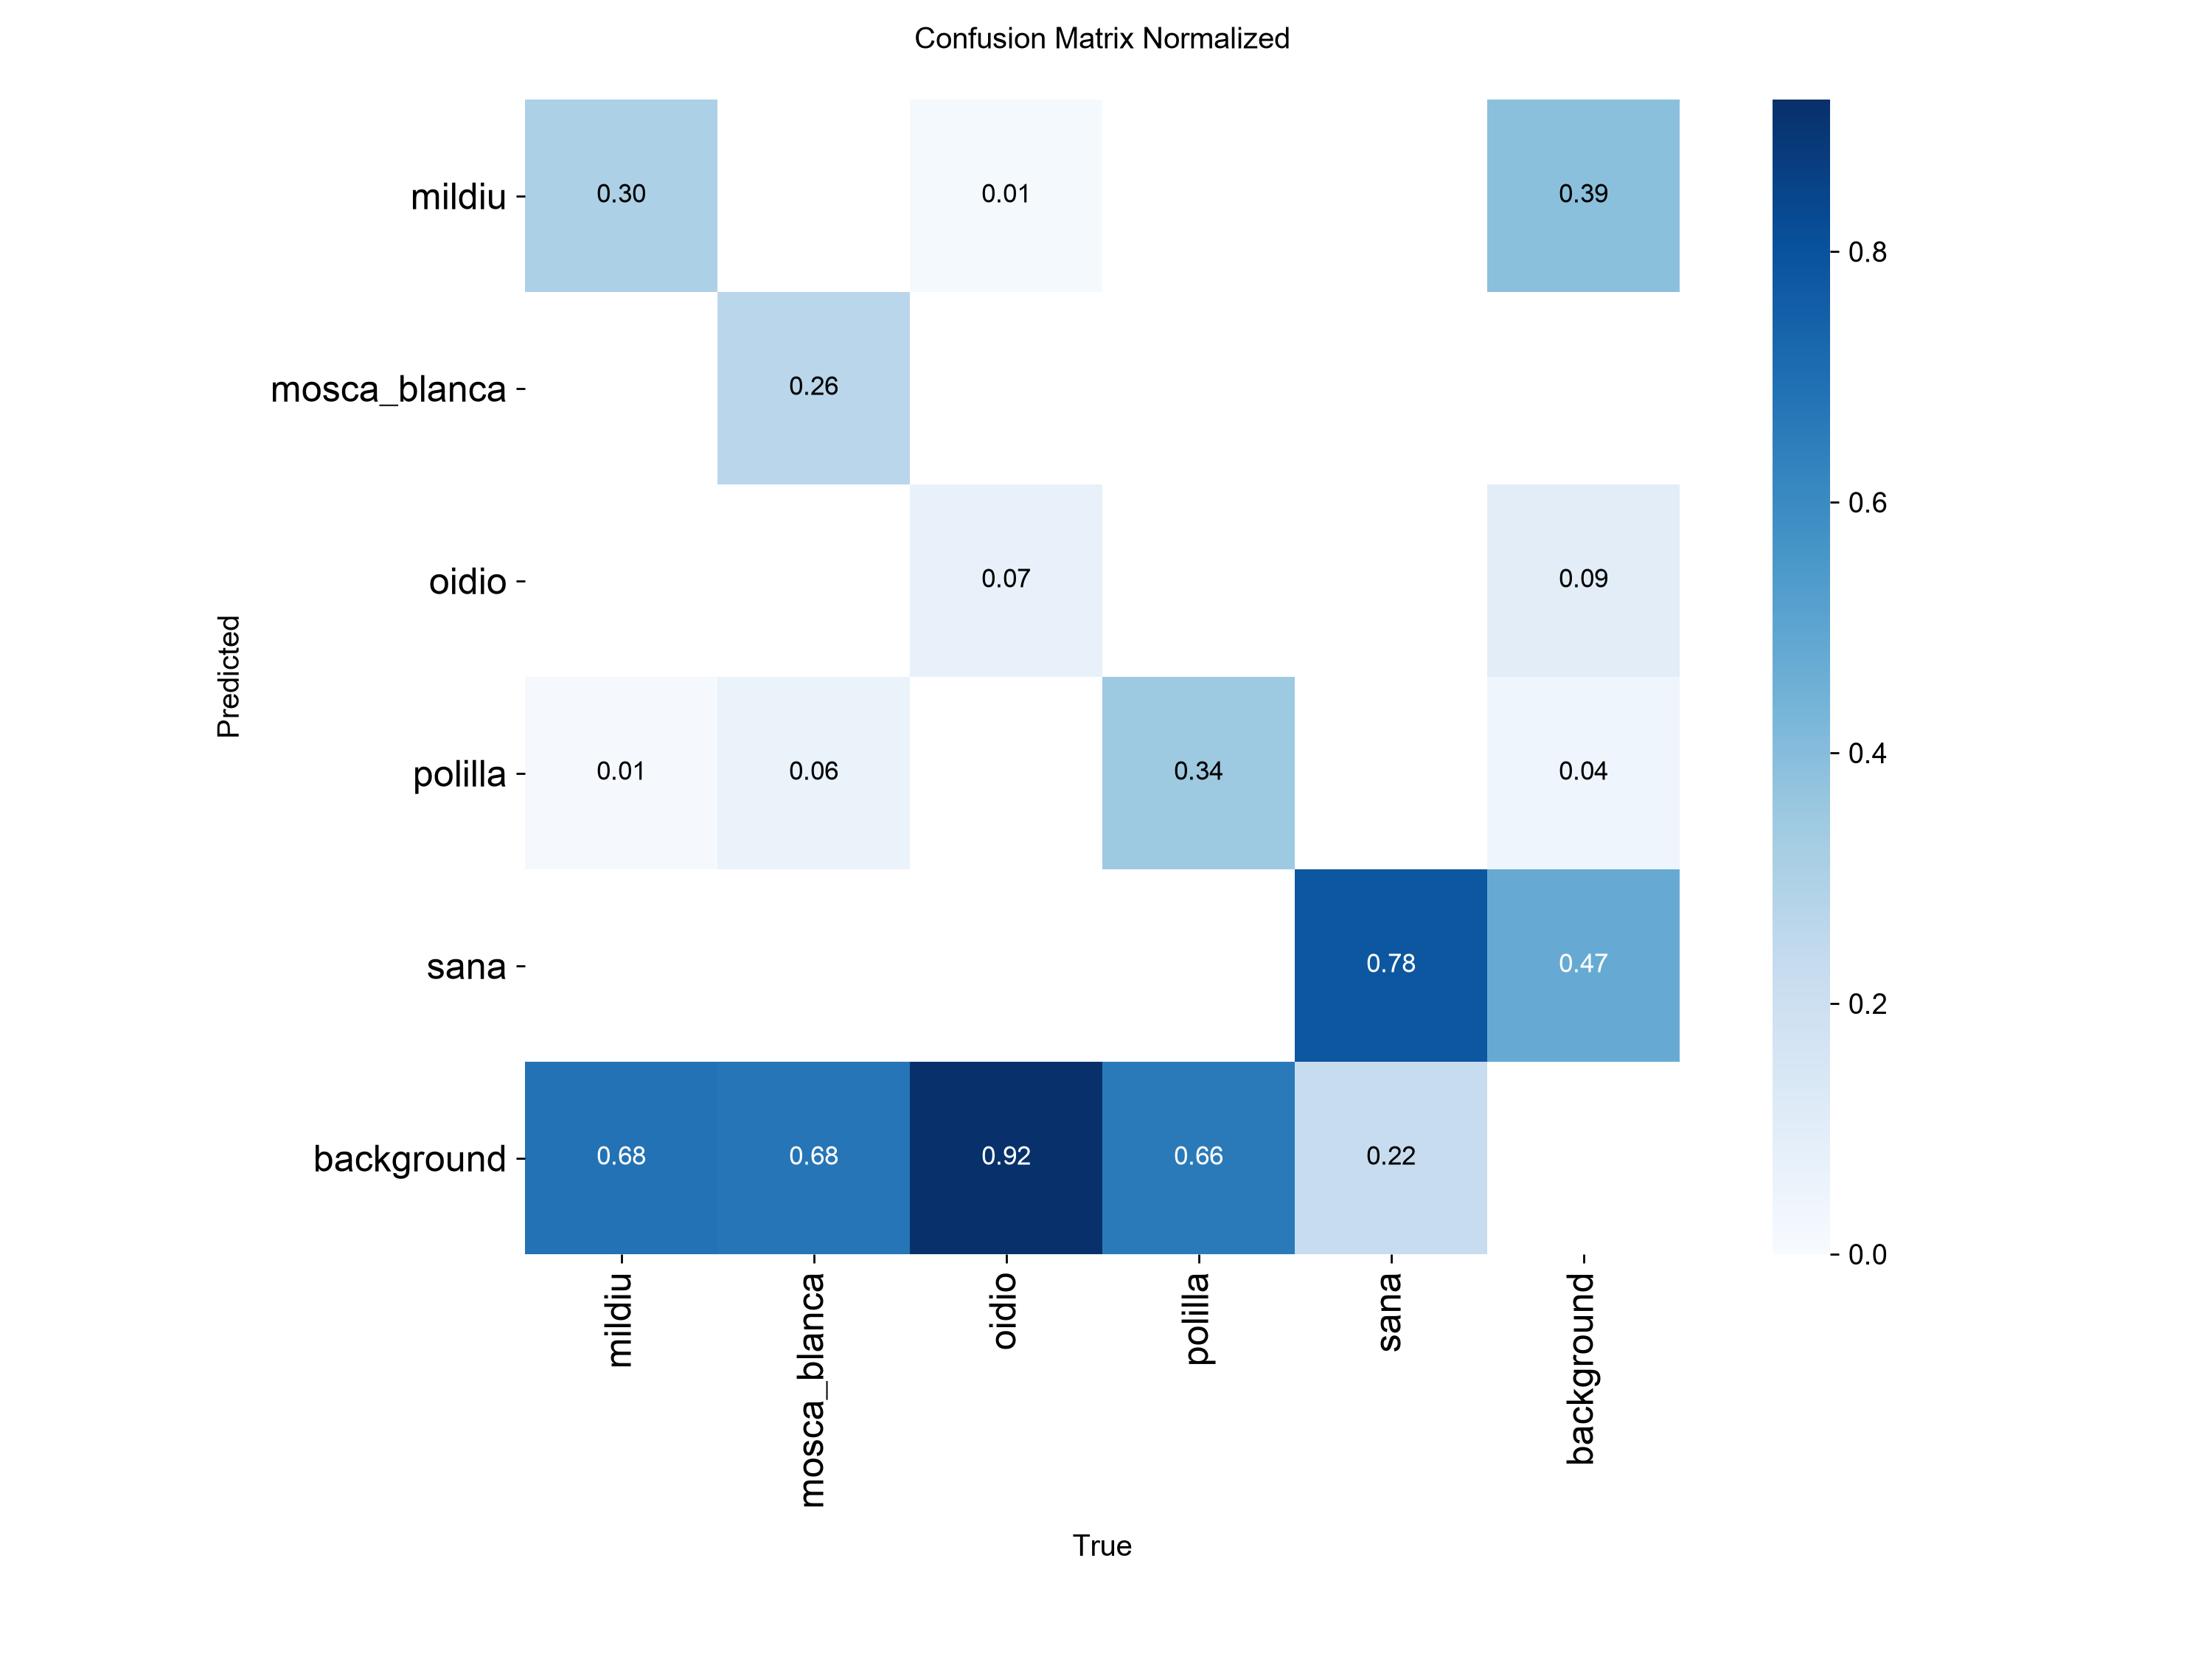
\includegraphics[width=0.40\textwidth]{cm_v5.png}\\
(a) & (b)
\end{tabular}
\caption{Modelo v5 (YOLOv8n, semilla 2): (a) curvas de pérdida y métricas; el mejor mAP@0.5:0.95 en validación se alcanza en la época 34 y la parada temprana corta en la 84; (b) matriz de confusión normalizada en la prueba.\label{fig:v5}}
\end{figure}

\subsection{Integración en el Móvil}

La Tabla~\ref{tab:movil} resume las pruebas en el teléfono con los modelos de la v1 y de la v4. Con la misma imagen de entrada, la versión TFLite y la ONNX difieren como máximo en 0.004 de confianza, y su detección principal coincide en 96 de 96 imágenes. La menor coincidencia con el servidor del modelo v4 (83.9\%) se debe a que sus confianzas quedan más cerca del umbral de 0.30, de modo que pequeñas diferencias al reducir la foto cambian cuál detección gana.

\begin{table}[H]
\caption{Pruebas en el Samsung Galaxy A56 con 192 imágenes de campo.\label{tab:movil}}
\begin{tabularx}{\textwidth}{lCC}
\toprule
\textbf{Prueba} & \textbf{Modelo v1 (YOLOv8n)} & \textbf{Modelo v4 (YOLO11n)}\\
\midrule
Tamaño TFLite float16 & 6.1 MB & 5.3 MB\\
Latencia por foto en el celular (P1) & $597 \pm 195$ ms & $501 \pm 120$ ms\\
Misma clase principal que el servidor (P2) & 94.3\% & 83.9\%\\
Cajas del servidor reproducidas (IoU $\geq 0.5$) & 78.3\% & 80.4\%\\
Servidor en CPU de laptop & $526 \pm 547$ ms & $205 \pm 38$ ms\\
Modo en vivo (P3) & $366 \pm 104$ ms/cuadro & ---\\
Fotos sin conexión sincronizadas (P4) & 5/5 & ---\\
\bottomrule
\end{tabularx}
\end{table}

El modelo de la v5 ya está instalado en el servidor (versión 3.0.0); en el teléfono sigue el TFLite de la v4 hasta repetir la conversión y las pruebas P1--P2. La Figura~\ref{fig:app} muestra la aplicación en funcionamiento.

\begin{figure}[H]
\centering
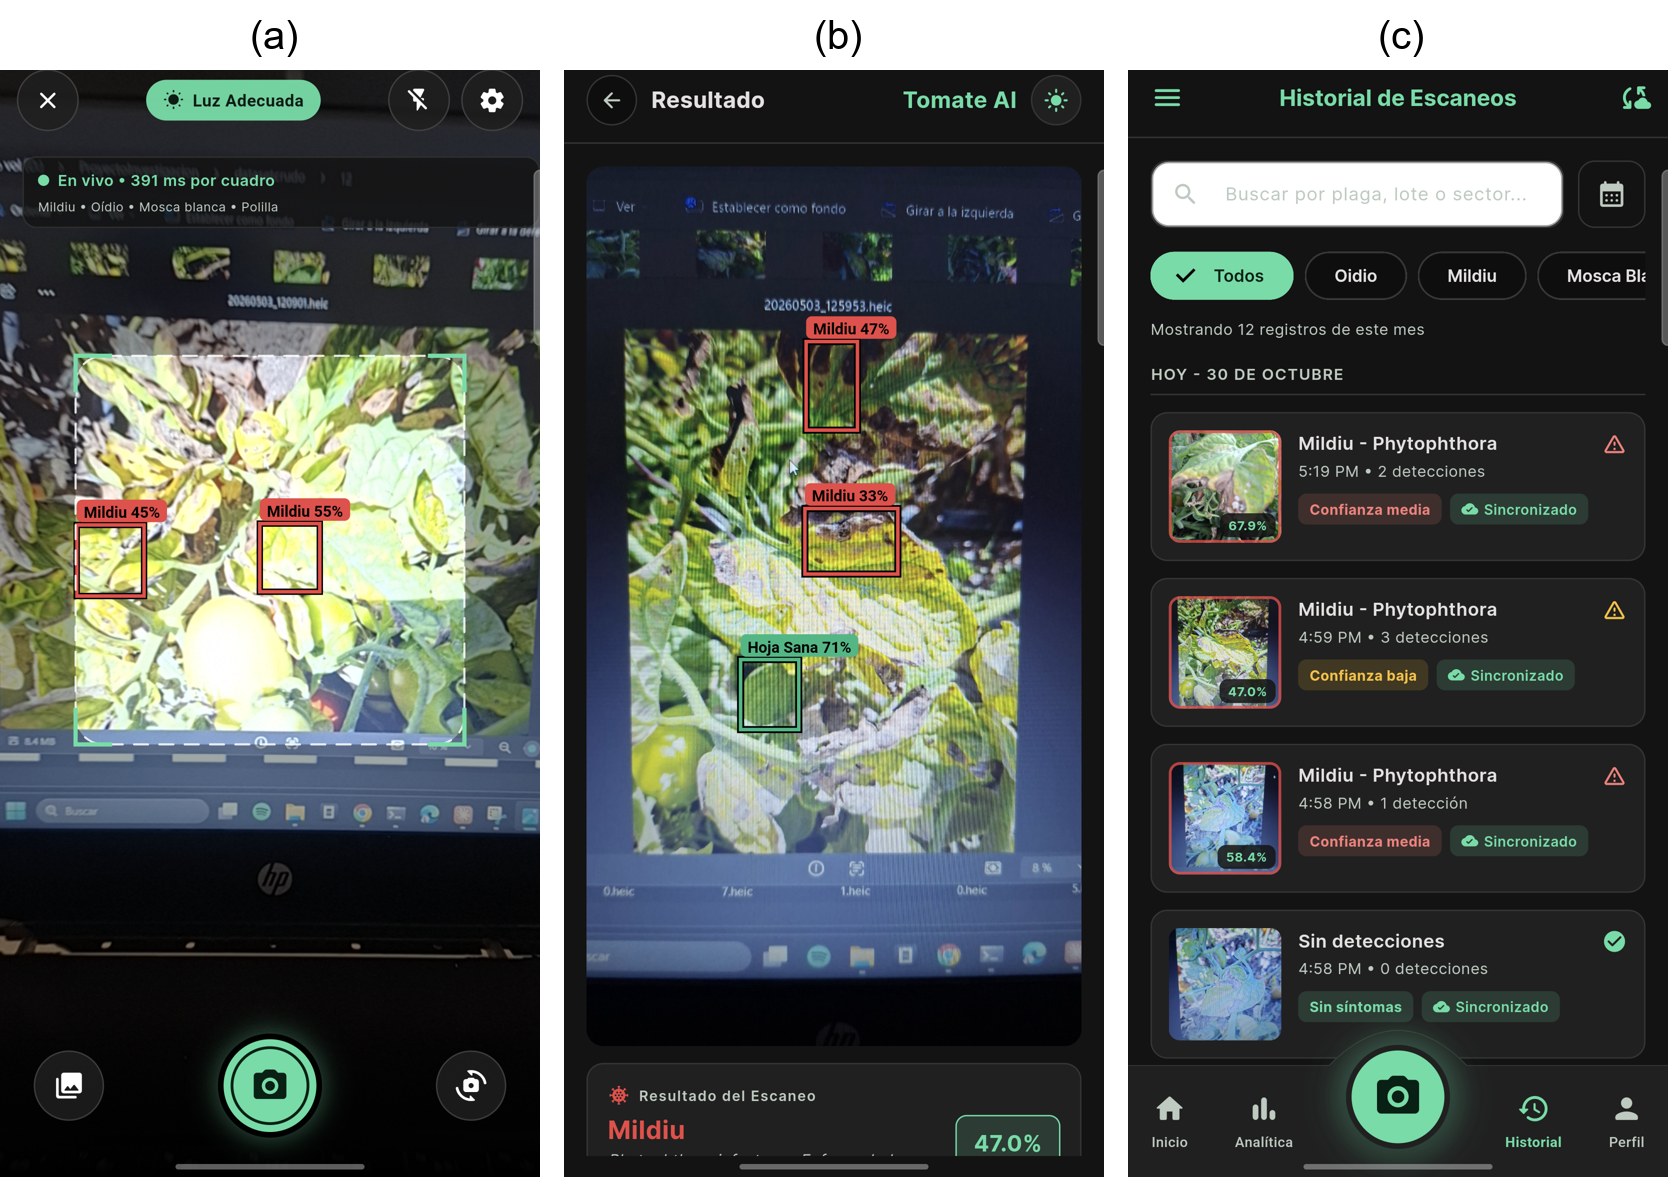
\includegraphics[width=0.9\textwidth]{fig_app_capturas.png}
\caption{Aplicación en el Samsung Galaxy A56: (a) modo en vivo con dos detecciones de mildiu (391~ms por cuadro); (b) resultado de una foto con mildiu y una hoja sana; (c) historial sincronizado con el servidor.\label{fig:app}}
\end{figure}

%=================================================================
\section{Discusión}

\textbf{La fuga de datos explicaba gran parte del resultado inicial.} Al pasar de la división por imagen a la división por planta, el mAP@0.5 en prueba bajó del 30\% de la v1 a un 21--24\%, y la polilla cayó de 65\% a 15--25\%. Medir la fuga con datos propios y corregirla fue la decisión metodológica más importante del trabajo~\cite{Kapoor2023}.

\textbf{Ampliar el dataset mejoró sobre todo la localización.} En las mismas imágenes de prueba, la v5 sube el mAP@0.5:0.95 en los tres modelos, es decir, sus cajas se ajustan mejor, pero el mAP@0.5 y el acierto del diagnóstico casi no cambian. Hay que considerar que entre la v4 y la v5 también cambiaron algunos hiperparámetros (\emph{batch}, tasa coseno, cierre del mosaico), por lo que la diferencia no se debe solo a los datos.

\textbf{Cada clase mejora según los datos nuevos que recibe.} Las tres clases cuyas cajas crecieron entre 93\% y 290\% mejoraron; oídio y mosca blanca, que crecieron 8\% y 23\%, empeoraron. Además, su proporción en el \emph{dataset} bajó (oídio pasó del 20\% al 11\% de las cajas de entrenamiento), lo que inclina al modelo hacia las clases mayoritarias. A esto se suma el tamaño: a 640~px la mosca blanca queda por debajo del tamaño que un detector puede resolver con fiabilidad~\cite{Zhang2024Jute}, y el polvo blanco del oídio es pequeño y difuso. El bajo AP de mildiu, pese a sus 1882 cajas, apunta más a lesiones que quedaron sin caja (en la v4, el 62\% de las detecciones falsas sobre el fondo eran ``mildiu'') y a su confusión con oídio, que deberá revisarse manualmente.

\textbf{Los tres modelos están empatados.} Las diferencias entre arquitecturas son del mismo tamaño que la variación entre semillas (hasta 6 puntos), y el mejor modelo cambia según se mire validación (YOLOv8n) o prueba (YOLOv10n). Con una sola semilla, como en la v1, no se habría podido elegir. Se mantiene YOLOv8n porque gana en validación, es el más rápido de entrenar y la aplicación ya procesa su formato de salida; YOLOv10n exigiría adaptar la aplicación.

\textbf{Más épocas o más GPU no ayudan.} El mejor modelo de cada corrida aparece entre las épocas 24 y 79 y luego la pérdida de validación sube. El límite está en los datos: 288 plantas de tres salidas al campo.

\textbf{Despliegue.} El modelo corre sin internet en unos 0.5~s por foto y los resultados se sincronizan al volver la conexión. Como la aplicación usa el mismo \emph{pipeline} para YOLOv8 y YOLO11, cambiar de modelo solo requiere convertirlo y repetir las pruebas.

%=================================================================
\section{Conclusiones y Trabajo Futuro}

Se completaron las Fases 1 a 4. El \emph{dataset} final tiene 1966 imágenes y 7766 anotaciones, dividido por planta y sin fuga de datos verificada. Los tres modelos ligeros evaluados quedan empatados, con un mAP@0.5 de 25--28\% en el test fijo y 32--36\% en la prueba completa, y un acierto de la clase principal cercano al 60\%. El sistema funciona en el servidor y sin conexión en el teléfono.

La principal conclusión es que el rendimiento está limitado por los datos y no por la arquitectura: las clases mejoran en proporción a los ejemplos nuevos, y oídio y mosca blanca necesitan más ejemplos y más resolución. El trabajo siguiente, en orden de impacto esperado, es:
\begin{itemize}[leftmargin=*,labelsep=4.9mm]
\item \textbf{Nueva salida al campo} con plantas nuevas, priorizando oídio, mosca blanca y polilla, e incluyendo el mediodía en otra fecha para el análisis de radiación. No se agregarán más cajas de \texttt{sana}, que ya son el 43\% del total.
\item \textbf{Revisión de etiquetas} de mildiu y oídio: lesiones sin caja y confusión entre ambas.
\item \textbf{Entrenamiento a $1024\times1024$}, que lleva la mosca blanca a unos 16~px, midiendo también la latencia en el teléfono.
\item \textbf{Conversión del modelo final a TFLite} y repetición de las pruebas P1--P5.
\end{itemize}

%=================================================================
\vspace{6pt}

\authorcontributions{Conceptualización, F.B.K.C. y H.J.C.C.; metodología, F.B.K.C. y H.J.C.C.; software, F.B.K.C.; investigación y curación de datos, F.B.K.C. y H.J.C.C.; redacción---borrador original, F.B.K.C.; redacción---revisión y edición, H.J.C.C. y A.R.C.C.; supervisión, A.R.C.C. Todos los autores han leído y aceptado la versión del manuscrito.}

\funding{Esta investigación no recibió financiamiento externo.}

\institutionalreview{No aplica.}

\informedconsent{No aplica.}

\dataavailability{El \emph{dataset} está disponible en Roboflow Universe con licencia CC~BY~4.0 (\url{https://universe.roboflow.com/fray-hxtls/plagas-tomate-majes-v2}). Los \emph{scripts} de curación, entrenamiento y evaluación, las métricas de cada corrida y los modelos entrenados están en \url{https://github.com/fraykanachullo/trabajoinvestigacionTomate}; el código del servidor y de la aplicación, en los repositorios indicados en la Tabla~\ref{tab:repro}.}

\acknowledgments{Agradecemos a los propietarios del Fundo El Pedregal (Majes) por el acceso al campo.}

\conflictsofinterest{Los autores declaran no tener conflictos de interés.}

%=================================================================
\begin{adjustwidth}{-\extralength}{0cm}
\reftitle{Referencias}
\begin{thebibliography}{999}

\bibitem[SENASA(2020)]{SENASA2020}
SENASA. Guía de Buenas Prácticas Agrícolas para el cultivo de tomate; Servicio Nacional de Sanidad Agraria: Lima, Perú, 2020. Disponible en: \url{https://www.senasa.gob.pe/senasa/descargasarchivos/2020/07/Guia-BPA-TOMATE.pdf}.

\bibitem[Mohanty et~al.(2016)]{Mohanty2016}
Mohanty, S.P.; Hughes, D.P.; Salath\'e, M. Using deep learning for image-based plant disease detection. {\em Front. Plant Sci.} {\bf 2016}, {\em 7}, 1419. \url{https://doi.org/10.3389/fpls.2016.01419}.

\bibitem[Jelali(2024)]{Jelali2024}
Jelali, M. Deep learning networks-based tomato disease and pest detection: A first review of research studies using real field datasets. {\em Front. Plant Sci.} {\bf 2024}, {\em 15}, 1493322. \url{https://doi.org/10.3389/fpls.2024.1493322}.

\bibitem[Fuentes et~al.(2017)]{Fuentes2017}
Fuentes, A.; Yoon, S.; Kim, S.C.; Park, D.S. A robust deep-learning-based detector for real-time tomato plant diseases and pests recognition. {\em Sensors} {\bf 2017}, {\em 17}, 2022. \url{https://doi.org/10.3390/s17092022}.

\bibitem[Zhong(2024)]{Zhong2024}
Zhong, Y. Tomato leaf disease identification based on YOLOv8. {\em Int. J. Comput. Sci. Inf. Technol.} {\bf 2024}, {\em 3}, 265--276. \url{https://doi.org/10.62051/ijcsit.v3n2.30}.

\bibitem[Wang and Liu(2025)]{Wang2025}
Wang, X.; Liu, J. TomatoGuard-YOLO: A novel efficient tomato disease detection method. {\em Front. Plant Sci.} {\bf 2025}, {\em 15}, 1499278. \url{https://doi.org/10.3389/fpls.2024.1499278}.

\bibitem[Mengesha and Mengistie(2025)]{Mengesha2025}
Mengesha, A.T.; Mengistie, M.A. Applying transfer learning in CNN model architectures for detecting tomato leaf disease with explainable artificial intelligence. {\em Smart Agric. Technol.} {\bf 2025}, {\em 11}, 101034. \url{https://doi.org/10.1016/j.atech.2025.101034}.

\bibitem[Yadav et~al.(2025)]{Yadav2025}
Yadav, R.; Seth, A.; Sharma, A.; Oza, M. Plant disease identification using deep learning and transfer learning. {\em Procedia Comput. Sci.} {\bf 2025}, {\em 260}, 341--352. \url{https://doi.org/10.1016/j.procs.2025.03.210}.

\bibitem[Zhang et~al.(2024)]{Zhang2024Jute}
Zhang, S.; Wang, H.; Zhang, C.; Liu, Z.; Jiang, Y.; Yu, L. JutePest-YOLO: A deep learning network for jute pest identification and detection. {\em IEEE Access} {\bf 2024}.

\bibitem[Das et~al.(2025)]{Das2025}
Das, A.; Pathan, F.; Jim, J.R.; Kabir, M.M.; Mridha, M.F. Deep learning-based classification, detection, and segmentation of tomato leaf diseases: A state-of-the-art review. {\em Artif. Intell. Agric.} {\bf 2025}, {\em 15}, 192--220. \url{https://doi.org/10.1016/j.aiia.2025.02.006}.

\bibitem[Shafi et~al.(2023)]{Shafi2023}
Shafi, U.; Mumtaz, R.; Qureshi, M.D.M.; Mahmood, Z.; Tanveer, S.K.; Haq, I.U.; Zaidi, S.M.H. Embedded AI for wheat yellow rust infection type classification. {\em IEEE Access} {\bf 2023}.

\bibitem[Ksibi et~al.(2022)]{Ksibi2022}
Ksibi, A.; Ayadi, M.; Soufiene, B.O.; Jamjoom, M.M.; Ullah, Z. MobiRes-Net: A hybrid deep learning model for detecting and classifying olive leaf diseases. {\em Appl. Sci.} {\bf 2022}.

\bibitem[Kapoor and Narayanan(2023)]{Kapoor2023}
Kapoor, S.; Narayanan, A. Leakage and the reproducibility crisis in machine-learning-based science. {\em Patterns} {\bf 2023}, {\em 4}, 100804. \url{https://doi.org/10.1016/j.patter.2023.100804}.

\bibitem[Jocher et~al.(2023)]{Jocher2023}
Jocher, G.; Chaurasia, A.; Qiu, J. Ultralytics YOLOv8, 2023. Disponible en: \url{https://github.com/ultralytics/ultralytics}.

\bibitem[Jocher and Qiu(2024)]{Jocher2024}
Jocher, G.; Qiu, J. Ultralytics YOLO11, 2024. Disponible en: \url{https://github.com/ultralytics/ultralytics}.

\bibitem[Wang et~al.(2024)]{Wang2024v10}
Wang, A.; Chen, H.; Liu, L.; Chen, K.; Lin, Z.; Han, J.; Ding, G. YOLOv10: Real-time end-to-end object detection. En {\em Advances in Neural Information Processing Systems 37 (NeurIPS 2024)}, 2024. \url{https://arxiv.org/abs/2405.14458}.

\bibitem[Kana Chullo(2026)]{Dataset2026}
Kana Chullo, F.B. plagas-tomate-majes-v2 Dataset. Roboflow Universe, 2026. Licencia CC BY 4.0. Disponible en: \url{https://universe.roboflow.com/fray-hxtls/plagas-tomate-majes-v2}.

\end{thebibliography}
\end{adjustwidth}
\end{document}
